\begin{comment}
------------------------------------------------------------------------------------------
\end{comment}
\chapter{RO-SLAM [new]}\label{ch:ro_slam}

Nachdem im vorherigen Kapitel die \Glspl{uwbm} für die Entfernungsmessung erstellt worden sind, wird jetzt nur noch eine Roboterplattform benötigt die mit einem Tag ausgestattet werden kann. Welche Hardwareplattform eingesetzt wird und von welchen Softwaremodulen diese gesteuert wird, folgt in den nächsten Abschnitten.

\begin{comment}
--------------------------------------------------------------------------------
- Einsatz mobiler Roboter in der Logistik am Beispiel des Robotino
	- http://www.r-moehrle.de/wissenschaftlicheArbeiten/robotino1.pdf
\end{comment}
\section{Roboterplattform [new]}

Um die Messungen für den \Gls{roslam} aufzuzeichnen wird eine Roboterplattform benötigt auf der das \Gls{uwbm} montiert werden kann. Zusätzlich wird noch eine Reihe weiterer Sensoren benötigt, die im Folgenden vorgestellt werden.

Also Roboterplattform dient dabei der Robotino 2 von \textit{Festo Didactic}. Er gehört zur Klasse der holonomen Roboter, d.h. seinen Bewegungsmöglichkeiten unterliegen keinerlei Einschränkungen im zweidimensionalen Raum. Ermöglicht wird das, durch drei voneinander unabhängig arbeitenden omnidirektionalen Antriebseinheiten. Jede der drei Antriebseinheiten verfügt über einen Inkrementalgeber, mit dem sich abschätzen lässt, wie weit der Robotino gefahren ist. Um den Fehler der Inkrementalgeber in Kurvenfahrten zu reduzieren wird das digitale Gyroskop\footnote{Model: CruizCore XG1000 / XG1010} von \textit{Microinfinity} eingesetzt. Gesteuert wird der Robotino über eine \SI{300}{\MHz} starke Verarbeitungseinheit auf Basis eines Linux Betriebssystems mit einem Echtzeitkernel. \cite{festo2007robotinomanual}

An der höchsten Position des Robotinos befindet sich ein 2D--Laser--Entfernungsmesser\footnote{Model: TiM571-2050101} der Firma \textit{Sick}. Mit einem Öffnungswinkel von \SI{270}{\degree} und einem Arbeitsbereich von \SIrange{0.05}{25}{\meter} ist es möglich, genaue Belegungskarten der Umgebung zu erstellen. \cite{sick2016operatingmanual}

Die Verarbeitungseinheit des Robotinos ist leistungsfähig genug um die anstehenden Steuerungsaufgaben zu erfüllen. Jedoch ist diese von leistungshungrigen Anwendungen wie dem \Gls{roslam} überfordert. Aus diesem Grund wird eine zusätzliche Verarbeitungseinheit\footnote{Model: NUC5i7RYH} mit einem Intel Core i7\footnote{5. Generation des Intel Core i7-5557U Prozessor mit bis zu \SI{3.4}{\GHz}. \cite{intel2015nucproductbrief}} verwendet.

Die Fahrbefehle werden dem Robotino über einen Xbox Wireless Controller übermittelt.

\begin{figure}[h]
	\centering
	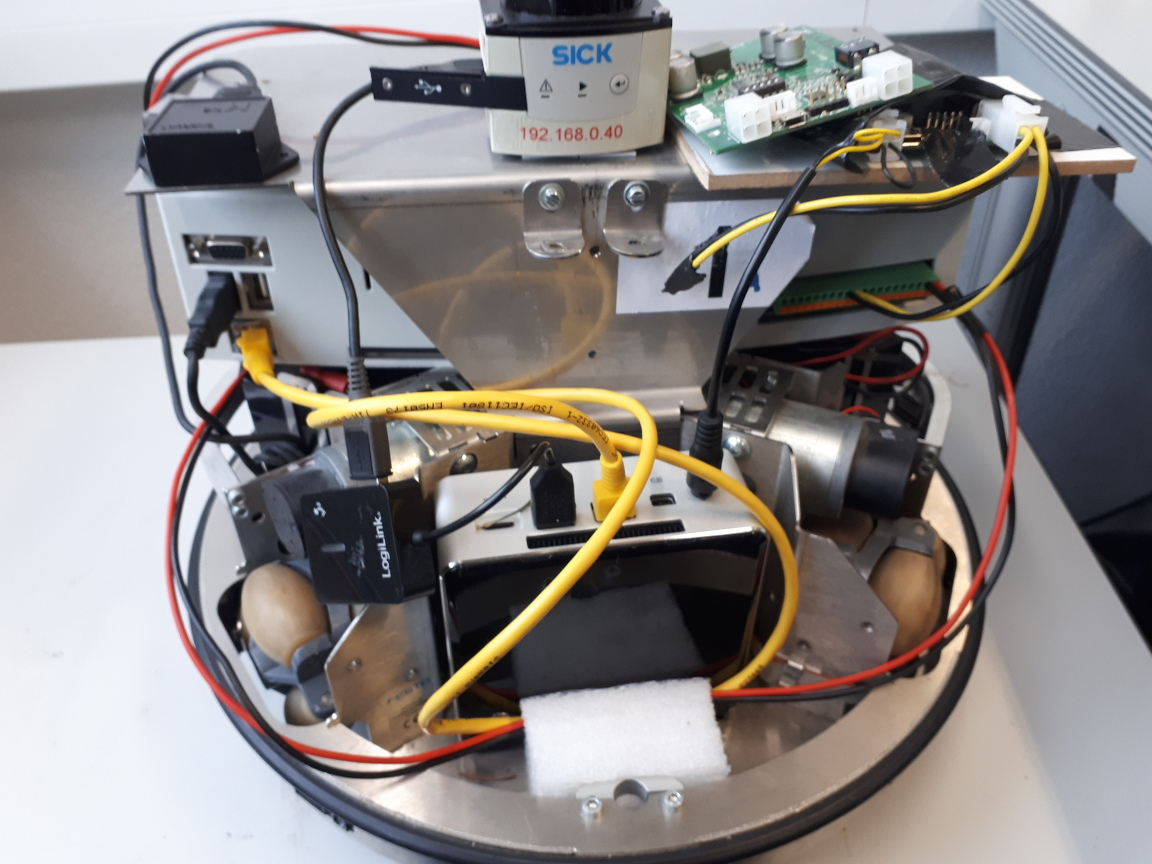
\includegraphics[width=0.5\textwidth]{robotino_front}
	\caption{[todo] Frontansicht des fertig aufgebauten Robotinos.}
	\label{fig:robotino_front}
\end{figure}


\begin{comment}
--------------------------------------------------------------------------------
- Kurzbeschreibung der Modulfunktion
- Welche Funktion erfüllt dieses Modul
- Welche ROS-Messages/-Topics/-Services bietet dieses Modul
\end{comment}
\section{Softwarearchitektur [new]}

Die Softwarearchitektur ist unterteilt in drei Bereiche. Die absolut notwendigen Module für den \Gls{roslam} werden in dem Abschnitt \Gls{ros}--Hauptmodule besprochen. In dem Abschnitt \Gls{ros}--Nebenmodule werden die Module besprochen, die im Nachgang für die Auswertung der Ergebnisse benötigt werden. Und im letzten Abschnitt wird das \Gls{mrpt}--Framework vorgestellt, das den \Gls{roslam}--Algorithmus bereitstellt.


\begin{comment}
--------------------------------------------------------------------------------
- todo: Übersicht über alle Module und deren Verbindung zu einander?
\end{comment}
\subsection{ROS--Hauptmodule [new]}


\begin{comment}
--------------------------------------------------------------------------------
- \url{http://wiki.ros.org/robotino_node}
- todo: Service reset_odometry
\end{comment}
\subsubsection{Robotino--Steuerung [new]}

Zur Steuerung der Roboterplattform muss die Verarbeitungseinheit Befehle zur Steuereinheit des Robotinos schicken. Diese Aufgabe erfüllt das \Gls{rosm} \textit{robotino\_node} aus dem Paket \textit{robotino\_node}. Über den Datenbus \textit{cmd\_vel} können die Geschwindigkeiten in X--/Y--Richtung und um die Z--Achse festgelegt werden. Um den Robotino zu stoppen, müssen alle drei Parameter auf den Wert Null gesetzt werden.

Um an die Informationen der Inkrementalgeber zu kommen muss das \Gls{rosm} \textit{robotino\_odometry\_node} aus dem Paket \textit{robotino\_node} gestartet werden. Nach dem Start steht der Datenbus \textit{odom} mit den aktuellen Werte der Inkrementalgeber zur Verfügung. Zusätzlich sorgt dieses Modul auch für die dynamische Transformation zwischen dem \textit{odom} und \textit{base\_link} Koordinatensystem.


\begin{comment}
--------------------------------------------------------------------------------
- \url{http://wiki.ros.org/robot_state_publisher}
- \url{http://wiki.ros.org/urdf}
\end{comment}
\subsubsection{Koordinatentransformation [new]}

Neben den dynamischen Transformationen besteht der Robotino auch aus vielen statischen Transformationen. Hierzu gehört z.B. die Transformation vom Robotino--Mittelpunkt zum 2D--Laser--Entfernungsmesser oder \Gls{uwbm}. Diese statischen Transformationen werden in einer \Gls{urdf}--Datei einmalig gespeichert und dann über das \Gls{rosm} \textit{state\_publisher} aus dem Paket \textit{robot\_state\_publisher} zur Laufzeit bereitgestellt, siehe \autoref{fig:rviz_robotino_tf2}.

\begin{figure}[h]
	\centering
	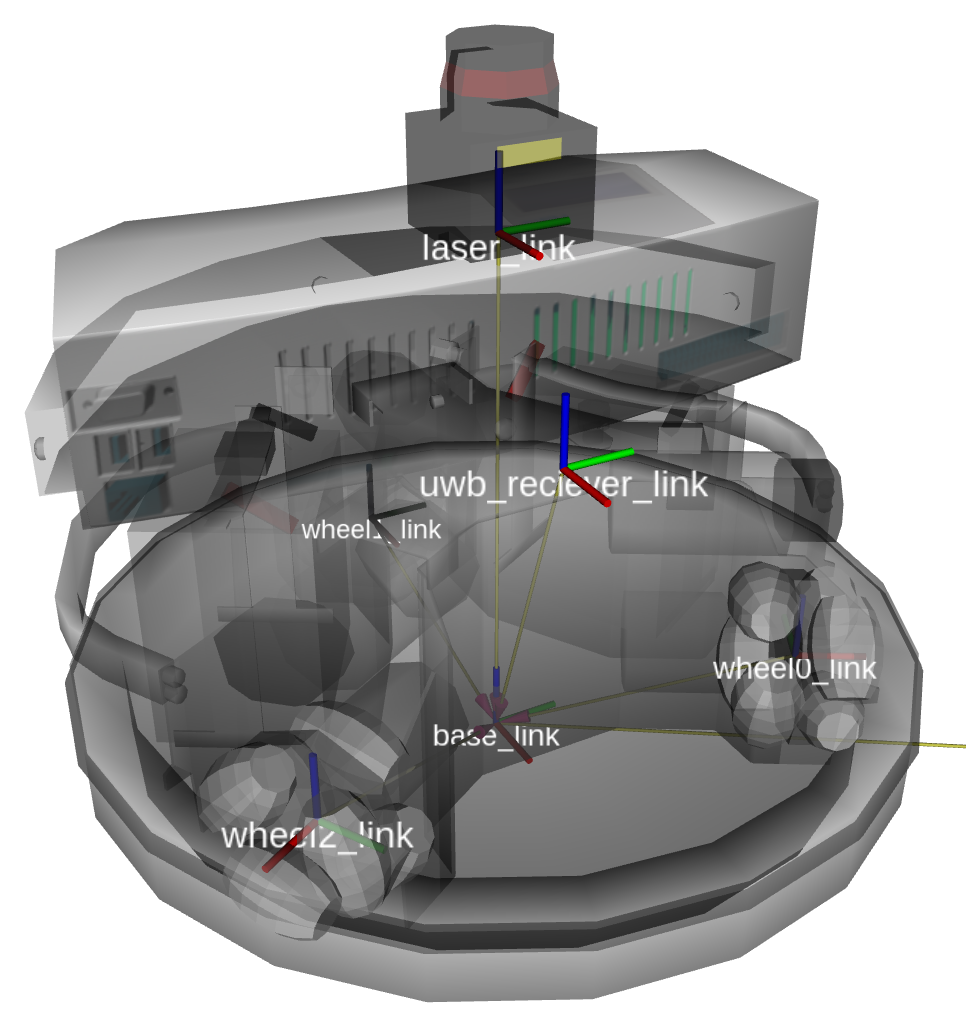
\includegraphics[width=0.5\linewidth]{rviz_robotino_tf2}
	\caption{Statische Transformationen des Robotino.}
	\label{fig:rviz_robotino_tf2}
\end{figure}


\begin{comment}
--------------------------------------------------------------------------------
- \url{http://wiki.ros.org/joy}
- todo: Referenz auf das lst:joy_node stehen lassen?
\end{comment}
\subsubsection{Teleoperation [new]}

Um die Roboterplattform zu steuern wird ein Eingabegerät benötigt. Ein \textit{Xbox Wireless Controller} wird dabei als Eingabegerät verwendet. Zustandsänderungen am Eingabegerät werden über das \Gls{rosm} \textit{joy\_node} aus dem Paket \textit{joy} registriert und über den Datenbus \textit{joy} bereitgestellt. Das überwachte Eingabegerät wird über den Parameter \textit{dev} festgelegt, siehe \autoref{lst:joy_node}.

Mit den generischen Daten des Eingabegerätes kann die Roboterplattform jedoch nichts anfangen, diese benötigt eine Nachricht vom Typ \textit{geometry\_msgs/Twist}. Die Transformation zwischen der Nachricht \textit{sensor\_msgs/Joy} und \textit{geometry\_msgs/Twist} erfolgt durch das \Gls{rosm} \textit{xbox\_teleop.py} aus dem Paket \textit{ro\_slam\_with\_uwb}.


\begin{comment}
--------------------------------------------------------------------------------
\end{comment}
\subsubsection{UWB--Abstandsmessungen [new]}

Die Abstandsmessungen zwischen dem \Gls{tag} und den vorhandenen \Glspl{anchor} werden durch das \Gls{uwbm} über die \Gls{usb}--Schnittstelle bereitgestellt. Die Daten werden dann von dem \Gls{rosm} \textit{beacon\_publisher.py} aus dem Paket \textit{ro\_slam\_with\_uwb} aufgefangen und auf den Datenbussen \textit{beacon} und \textit{beacon\_raw} veröffentlicht. Der erste Datenbus ist vom Typ \textit{mrpt\_msgs/ObservationRangeBeacon} und wird von dem \Gls{mrpt}--Modul für den \Gls{roslam} benötigt. Der zweite Datenbus wird für die Auswertung der Abstandmessungen im \autoref{ch:eval} benötigt und ist vom Typ \textit{ro\_slam\_with\_uwb/Beacon}.


\begin{comment}
--------------------------------------------------------------------------------
\end{comment}
\subsection{ROS--Hilfsmodule [new]}


\begin{comment}
--------------------------------------------------------------------------------
- \url{http://wiki.ros.org/sick_tim}
\end{comment}
\subsubsection{2D--Laser--Entfernungsmesser [new]}

Der 2D--Laser--Entfernungsmesser gehört zu einem der am häufigsten verwendeten Sensoren für die präzise visuelle Erfassen der Umwelt. Für mehrere der nachfolgenden \Gls{rosm} ist eine 2D--Laser--Entfernungsmessung eine zwingende Voraussetzung. Um die Daten dem \Gls{ros}--System bereitzustellen wird das \Gls{rosm} \textit{sick\_tim551\_2050001} aus dem Paket \textit{sick\_tim} verwendet. Dieses Modul stellt über den Datenbus \textit{scan}, mit einer Rate von \SI{15}{\hertz}, Nachrichten vom Typ \textit{sensor\_msgs/LaserScan} bereit.


\begin{comment}
--------------------------------------------------------------------------------
- \url{http://wiki.ros.org/hector_mapping}
\end{comment}
\subsubsection{Belegungskarten [new]}

Das erste \Gls{rosm}, das von der 2D--Laser--Entfernungsmessung Gebrauch macht, ist das \textit{hector\_mapping} aus dem Paket \textit{hector\_mapping}. Mit diesem Modul können präzise Belegungskarten (engl. Occupancy Grid Map) erstellt werden, die für jede Koordinate der Karte festlegen ob diese durch ein Hindernis belegt (schwarz) oder frei (weiß) ist. Bereiche die von Hindernissen verdeckt sind oder außerhalb der Sensorreichweite liegen, werden als unbestimmt (grau) markiert, siehe \autoref{fig:rviz_occupancy_grid_map}. In \Gls{ros} werden Belegungskarten mit dem Nachrichtentyp \textit{nav\_msgs/OccupancyGrid} repräsentiert.

Zu den wichtigsten Parametern zählt die minimale und maximale Sensorreichweite (\textit{laser\_min\_dist} bzw. \textit{laser\_max\_dist}) die für die Kartenerstellung berücksichtigt wird und die Auflösung (\textit{map\_resolution}) einer Zelle in der Karte.

\begin{figure}[h]
	\centering
	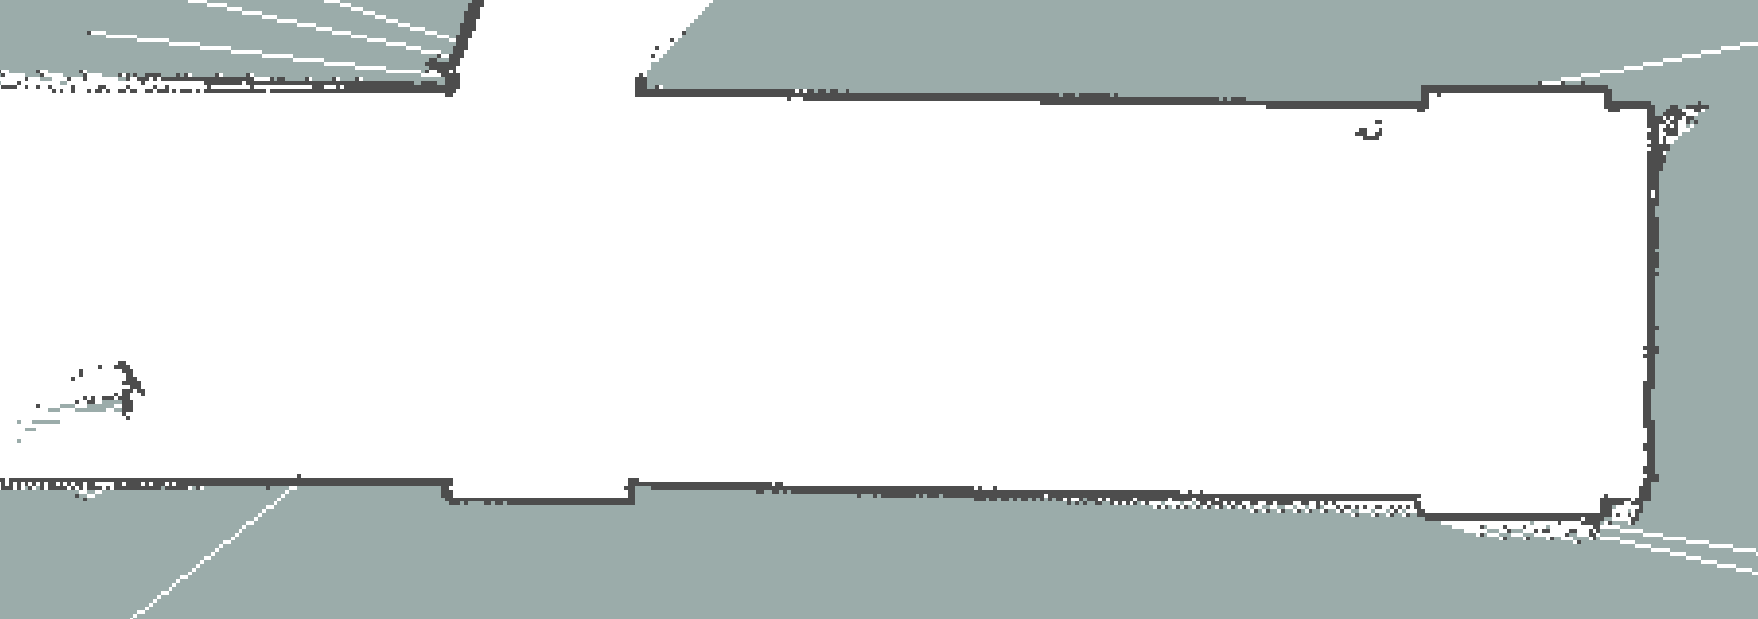
\includegraphics[width=0.9\linewidth]{rviz_occupancy_grid_map}
	\caption{Die Belegungskarte der Messstrecke.}
	\label{fig:rviz_occupancy_grid_map}
\end{figure}
 

\begin{comment}
--------------------------------------------------------------------------------
- \url{http://wiki.ros.org/hector_trajectory_server}
- \url{http://docs.ros.org/api/nav_msgs/html/msg/Path.html}
\end{comment}
\subsubsection{Trajektorie [new]}

Neben den Entfernungsinformationen wertet der \Gls{roslam} auch die Daten der Odometrie aus. Als Quelle für die Odometrie dienen dabei die Inkrementalgeber des Robotino. Im nächsten Abschnitt werden weitere Quellen für die Odometrie vorgestellt. Um die Güte der Odometrie--Quellen zu vergleichen, wird die verfahrene Trajektorie jeder Quelle benötigt. Diese Informationen werden von dem \Gls{rosm} \textit{hector\_trajectory\_server} aus dem Paket {hector\_trajectory\_server} bereitgestellt. Die Daten liegen dabei als Nachricht vom Typ \textit{nav\_msgs/Path} bereit und können in die Belegungskarte integriert werden, siehe \autoref{fig:rviz_trajektorie}.

\begin{figure}[h]
	\centering
	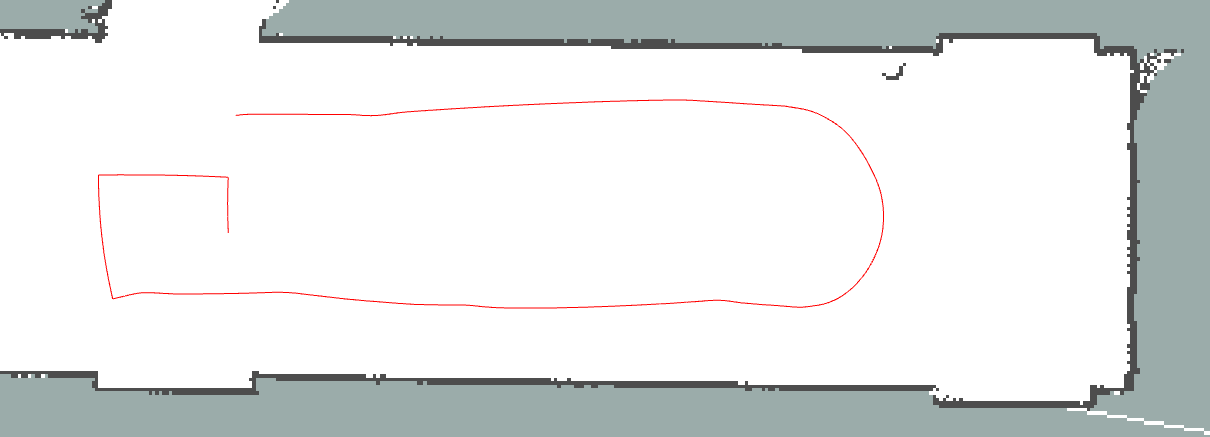
\includegraphics[width=0.9\linewidth]{rviz_trajektorie}
	\caption{Die Trajektorie einer Messfahrt des Robotino.}
	\label{fig:rviz_trajektorie}
\end{figure}


\begin{comment}
--------------------------------------------------------------------------------
- \url{http://wiki.ros.org/rf2o}
- \url{http://wiki.ros.org/laser_scan_matcher}
\end{comment}
\subsubsection{Laser--Odometrie [new]}

Wie bereits im vorherigen Abschnitt erwähnt, werden hier zwei weitere Quelle für die Odometrie vorgestellt. Beide \Glspl{rosm} nutzen nur die Daten der 2D--Laser--Ent\-fern\-ungs\-mes\-sung um eine Schätzung für die aktuelle Pose zu erstellen. Bei dem ersten handelt es sich um den \textit{laser\_scan\_matcher\_node} aus dem Paket \textit{laser\_scan\_matcher} und bei dem zweiten um den \textit{rf2o\_laser\_odometry\_node} aus dem Paket \textit{rf2o\_laser\_odometry}.


\begin{comment}
--------------------------------------------------------------------------------
- \url{https://www.mrpt.org}
- \url{http://wiki.ros.org/mrpt_slam}
- \url{http://wiki.ros.org/mrpt_navigation}
- \url{https://www.mrpt.org/tutorials/slam-algorithms/rangeonly_slam/}
	- Bayesian range-only SLAM (RO-SLAM) with SOGs
- \url{http://mrpt.ual.es/reference/devel/classmrpt_1_1slam_1_1_c_metric_map_builder_r_b_p_f.html}
	-mrpt::slam::CMetricMapBuilderRBPF Class Reference
	- It is actually a front-end to the class mrpt::slam::CMetricMapBuilderRBPF. All the parameters to the algorithm are passed through a configuration file in the command line. The filter processes actions and observations from a rawlog file and optionally generates a number of files describing the evolution of the filter and the maps.
\end{comment}
\subsection{MRPT [new]}

Bei dem \Gls{mrpt}--Framework handelt es sich um eine Bibliothek die Datenstrukturen und Algorithmen aus dem aktiven Forschungsbereich der Robotik bereitstellt. Dadurch ist eine schnelle Umsetzung neuer Algorithmen, sowie der Vergleich mit bereits bestehenden möglich. Zu den verfügbaren Datenstrukturen zählen die Basisdatentypen der linearen Algebra bis hin zu den komplexeren Datentypen der Robotik wie z.B. die Belegungskarten. Zur direkten Verwendung existieren viele Algorithmen aus den Bereichen der \Gls{slam}--Algorithmen, des Maschinellen Sehen (engl. Computer Vision) und der Pfad-- und Bewegungsplanung (engl. Path/Motion Planning).

Aus dem Bereich der \Gls{roslam}--Algorithmen sind die Verfahren aus den Veröffentlichungen \citetitle{blanco2008pure} und \citetitle{blanco2008efficient} implementiert, siehe \autoref{sec:blanco2008pure} und \ref{sec:blanco2008efficient}.

Um die \Gls{roslam}--Algorithmen aus dem \Gls{mrpt}--Framework zu nutzen, wird das \Gls{rosm} \textit{mrpt\_rbpf\_slam} aus dem Paket \textit{mrpt\_rbpf\_slam} benötigt. Mit dem Parameter \textit{ini\_filename} wird der Dateipfad zu der Konfigurationdatei für die \Gls{roslam}--Algorithmen angegeben und über den \textit{sensor\_source} Parameter werden die Datenquellen für den \Gls{roslam} definiert. Hierbei ist es möglich sowohl die Entfernungsmessungen der \Gls{uwbm} als auch die der 2D--Laser--Entfernungsmesser anzugeben. Von der letzten Datenquelle wird kein gebraucht gemacht, da dadurch Transformationen zwischen Koordinatensystemen veröffentlicht werden die mit den bereits bestehenden kollidieren. Über die Datenbusse \textit{particlecloud} und \textit{particlecloud\_beacons} werden die Positionsschätzungen für den Roboter und die \Glspl{uwbm} veröffentlicht, siehe \autoref{fig:rviz_robot_and_beacon_estimate}.

\begin{figure}[h]
	\centering
	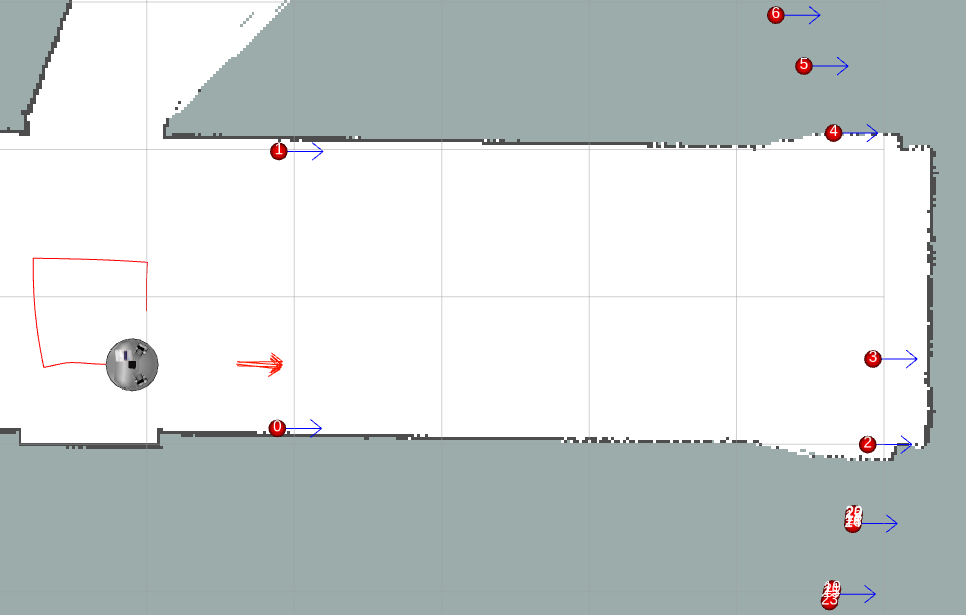
\includegraphics[width=0.9\linewidth]{rviz_robot_and_beacon_estimate}
	\caption{Positionsschätzung für den Roboter mit roten Pfeilen und für die \Glspl{uwbm} mit grünen Pfeilen.}
	\label{fig:rviz_robot_and_beacon_estimate}
\end{figure}

Nach der Konfiguration der \Gls{ros} Seite müssen noch Einstellungen für den \Gls{roslam} festgelegt werden. Hier muss die Konfigurationsdatei, die in dem \Gls{ros}--Parameter \textit{ini\_filename} hinterlegt ist, bearbeitet werden. Das \Gls{mrpt}--Framework verfügt über einen eigenen Abspielmechanismus für aufgezeichnete Messungen. Dieser wird nicht verwendet, da \Gls{ros} über einen eigenen Mechanismus verfügt. Folglich wird der Parameter \textit{rawlog\_file=} auf einen leeren Wert gesetzt werden. Auch verfügt \Gls{ros} über eine eigene Visualisierungslösung, daher wird die grafische Anzeige des \Gls{mrpt}--Frameworks über den Parameter \textit{SHOW\_PROGRESS\_IN\_WINDOW=0} deaktiviert. Um zwischen den beiden \Gls{roslam}--Verfahren zu wechseln, wird der Parameter \textit{insertAsMonteCarlo} angepasst werden.

